\documentclass[smallextended]{svjour3}
\usepackage{mathptmx}
\usepackage{graphicx}
\begin{document}
\title{Distributed, agent-based equilibrium solution with iterative network
updates}
\author{David Prentiss}
\institute{David Prentiss \at
  George Mason University
  \email{dprentiss@gmail.com}
}
\date{\today}
\maketitle
\begin{abstract}
  We propose an agent based model for approximating the competitive
  equilibrium for exchange economies. Our model employs simple agents
  engaged in bilateral trade in a network. Highly parallel agent algorithms and
  minimal graph operations allow for agents to trade to equilibrium over many
  different network topologies. We employ the wealth effect alone to guide our
  search in a large space of possible topologies.
\end{abstract}
\section{Introduction}
  \begin{itemize}
  \item \cite{albin1992decentralized}: Agents trade two goods with partners found by
    broadcasting interests.
  \item \cite{wilhite2001bilateral}: The effects of different network
  topologies on agents engaged in bilateral trade.
  \item \cite{sunder2002simple}: An iterative scheme where traders retain
  price information from previous epochs of trading.
  \item \cite{axtell2005complexity}: Agents trading bilaterally are more
    efficient than the Walrasian process for large numbers of goods and agents.
  \item What if we used wealth effects to update trading partners iteratively?
  \end{itemize}
\section{Model}
Our model is comprised of simple agents in a pure exchange economy.
These agents exchange abstract goods with neighboring agents in a network.
Each node of the network represents a single agent with adjacent edges defining
its neighbors.
Trade proceeds in discrete rounds in which agents may make and/or accept a bid
from each of its neighbors.
When a sequence of rounds results in agents having exhausted all trading
opportunities, we call that sequence an epoch.
At the close of each epoch, the network topology is modified, agents'
endowments are reinstated, and trade begins again.
As such, trading epochs continue in sequence until an exogenous stopping
criterion is met.
The rest of this section describes agents, the network, and network
modifications in greater detail.

\subsection{Agents}
Following \cite{albin1992decentralized}, agent's endowments are sampled from a uniform distribution such that there is an equal amount of each good in the economy and the unit sum of goods for each trader is 100.
Additionally, agents' preferences are represented by a symmetrical, Cobb-Douglas utility function.
As a result, the optimal marginal rates of substitution for both goods are one.

Agents may exchange goods only with their immediate neighbors and are privy to their
neighbors' respective marginal rates of substitution. Each round, every agent
completes actions in the following order:
\begin{enumerate}
\item Check if the bid from the previous round were accepted.
If a previous bid was accepted by a neighbor, update allocation and MRS.
\item Consider bids from neighbors and accept all rational offers.
Bids are rational if the exchange improves the agents utility. If a bid is
accepted, update allocation and MRS.
\item Make the best offer to a single neighbor.
\end{enumerate}

Agents do not learn or otherwise retain information from past epochs.
The only mechanism by which agents might act differently from one epoch to the next is
a change in the set of other agents available for trade, i.e. a change in
network topology.

\subsection{Network}
The network is comprised of one node per agent and the edges that connect them.
Network topology is initially a ring with each agent having two neighbors.
This topology is altered by successive epochs as edges are added and removed.
When each epoch is completed, the network update heuristic is executed. In this work
we considered two update heuristics: one which only adds new edges and another
which both adds and removes edges.

\subsubsection{Add-only Network Update Heuristic}
  At the end of each epoch:
  \begin{enumerate}
  \item Identify worst-off agent
  \item Add edge to next-worst-off agent that is not already a neighbor
  \item Stop when graph is complete
  \end{enumerate}
\subsubsection{Add-and-remove Network Update Heuristic}
  At the end of each epoch:
  \begin{enumerate}
  \item Identify worst-off agent
  \item Add edge to random agent that is not already a neighbor
  \item Randomly remove an edge connecting agents that both have two or more neighbors
  \item Stop after an arbitrary number of epochs.
  \end{enumerate}

\subsection{Implementation}
One of the principles guiding this research was the computational independence
of agents. Ideally, each agent would be able to take its actions based on
locally stored data and without regard for the actions taken simultaneously by
other agents.
To this end, agents to not communicate with their neighbors during a round.
Instead, a bid made by an agent in one round are placed in shared memory and
considered by that agents neighbor at the beginning of the following round.
Regardless of whether a bid made to any particular neighbor, each agent places
its MRS in shared memory for used by all of its neighbors in formulating their
bids.
While in this work agents exhibit very simple behavior relatively little market
data, in principle, more complex agents could be implemented while preserving
their computational independence.
The purpose of this choice was to allow for parallel execution of agent
functions.

The model is built in MASON, an agent-based modeling and visualization
library implemented in Java. Agents are ordinary Java objects while the network
is a graph object provided by MASON. In concept the network graph is undirected.
However, it is implemented with pairs of directed edges in order to distinguish incoming
and outgoing bids from each pair of neighboring agents. As such the network
object consists only of references to agent objects and the most recent MRS and
bids from each agent. Although, it contains multiple copies of each, depending
on the number neighbors each agent has.

\section{Simulation Results}
The add-only heuristic was first to be implemented and tested. Economies with up
to 512 agents were run with randomly generated endowments. In most cases the
simulation was run until all agents in the network were fully connected.
Here we illustrate our results with a typical example with 64 agents.
Figure \ref{h1start} shows the result for our example.
For the add-only heuristic, initial epochs reduced the wealth effect but
increased connectivity in the network tended to increase it. Figure
\ref{h1allgap} shows the maximum and minimum wealth changes for the same example.
The equilibrium prices were found quickly and stable until termination.
Figures \ref{h1prices} and \ref{h1allpricesave} show the MRS with respect to
good to for each agent and the average respectively.

With the add-only heuristic, agents quickly found the equilibrium price and
consistently reduces the wealth effect in early epochs. However, it's tendency
to increase the wealth effect over successive epochs, while an interesting
result in and of itself, rules it out as a candidate for our purposes.
In addition to this drawback, fully connected agents take a relatively large
number of operations to process each round in large networks. If executed purely
in parallel this would not necessarily be a practical issue. However with
minimal paralellization, large networks become infeasible.

\begin{figure}
  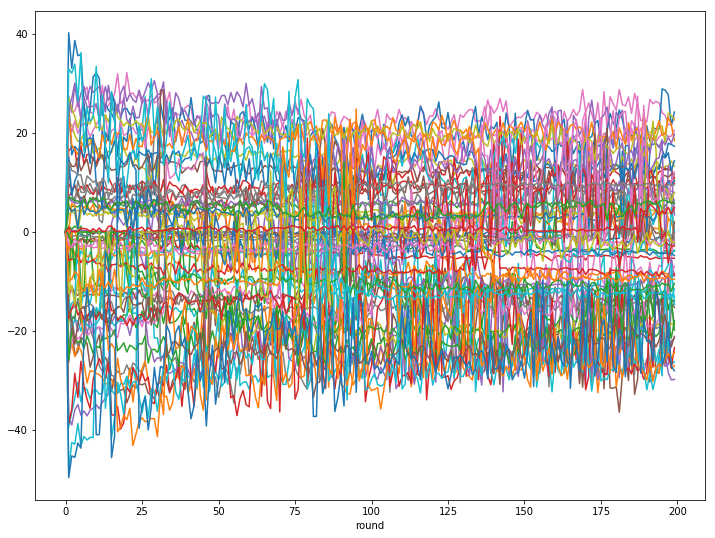
\includegraphics[width=0.75\textwidth]{h1startwealth.png}
  \caption{Wealth effect after each epoch for a typical, 64-agent example with the add-only
    network update heuristic. }
  \label{h1start}
\end{figure}

\begin{figure}
  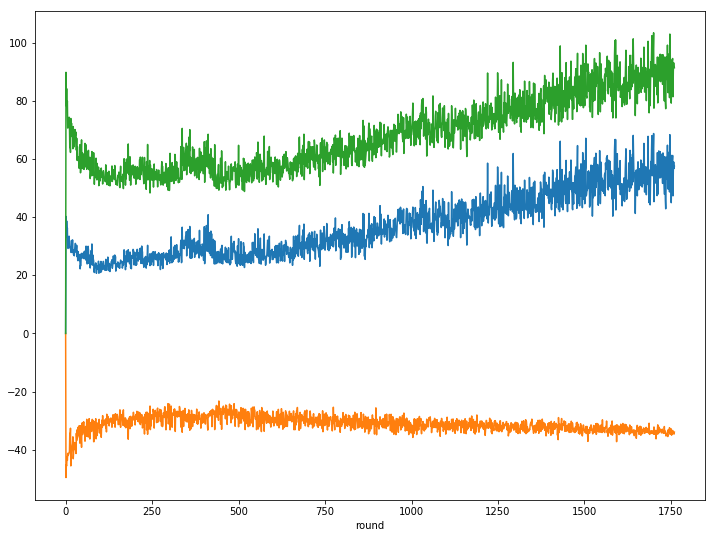
\includegraphics[width=0.75\textwidth]{h1allgap.png}
  \caption{Extrema of wealth effect after each epoch for a typical, 64-agent
    example with the add-only network update heuristic. The maximum (blue),
    minimum (orange), and difference (green) are shown.}
  \label{h1allgap}
\end{figure}

\begin{figure}
  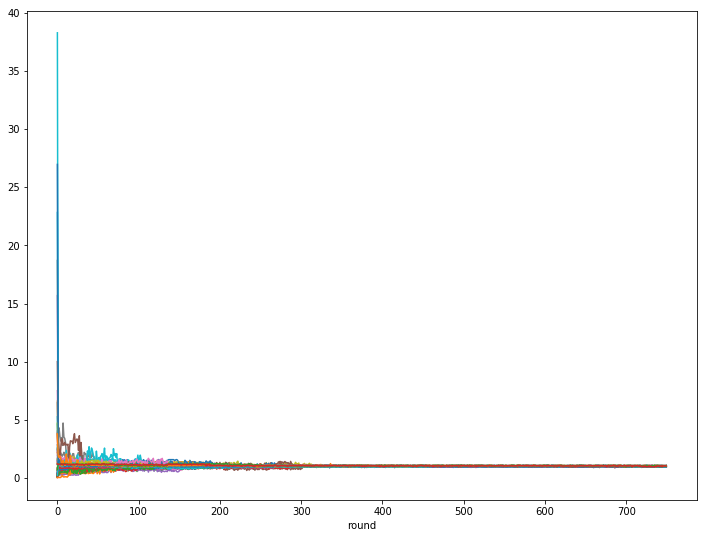
\includegraphics[width=0.75\textwidth]{h1prices.png}
  \caption{MRS of good two with respect to good one (numeraire) after each epoch
    for a typical, 64-agent example with the add-only network update heuristic.
    Each color represents a different agent}
  \label{h1prices}
\end{figure}

\begin{figure}
  \caption{Average MRS of good two with respect to good one (numeraire) after each epoch for a typical, 64-agent example with the add-only network update heuristic. }
  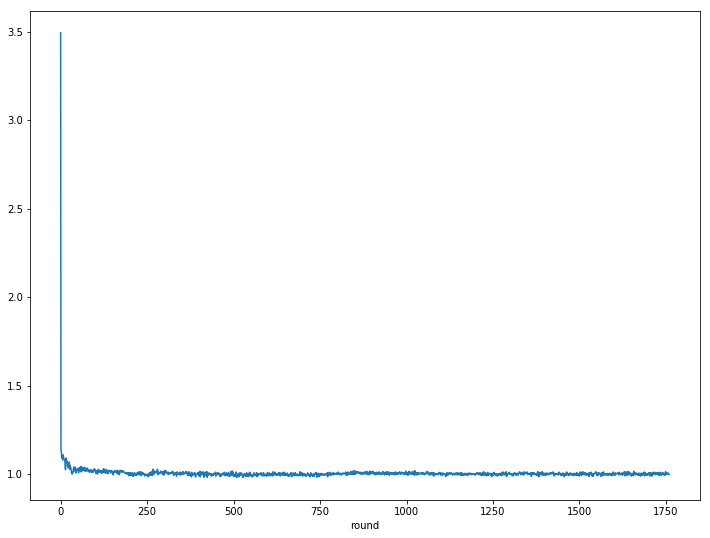
\includegraphics[width=0.75\textwidth]{h1allpriceave.png}
  \label{h1allpriceave}
\end{figure}

%\begin{figure}
  %\caption{Wealth effect after each epoch for a typical, 64-agent example with the add-only
    %network update heuristic. Results near the lowest wealth change achieved in
    %this example are shown.}
  %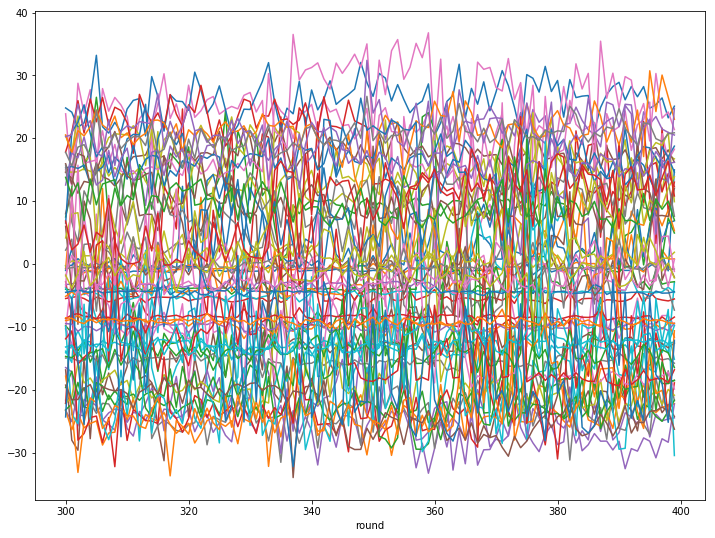
\includegraphics[width=\textwidth]{h1bestwealth.png}
%\end{figure}

The next update heuristic to be considered allow for edges to be removed.
Compared with the add-only heuristic this method was more computationally
efficient and found a network configuration with a lower wealth effect for the
same endowment. Again, we illustrate our results here with the same initial economy
demonstrated for the add-only heuristic.
Figure \ref{h2startwealth} shows the wealth effect for the first 200 epochs
and figure \ref{h2startgap} shows the wealth effect extrema for the 64-agent example.
In general, the add-and-remove finds better solutions in less time but
not necessarily in fewer epochs.
However, this advantage is mitigated by several drawbacks.

First, our simulations failed to demonstrate a significant trend to convergence after a few
thousand epochs. Figure \ref{h2allgap} shows the wealth effect extrema for 8000
epochs in our example. While successive epochs do not diverge as with the
add-only heuristic, they show no convergent trend.

Second, prices (MRS) are not as stable. This is the direct result of the
heuristic in that there is no guarantee that the entire network will stay
connected.
On the contrary, the price spikes shown in \ref{h2prices} and \ref{h2allpriceave} illustrate a common
state of affairs where small sections of the network, sometimes as small as one agent,
become disconnected and agent cannot rationally trade. In this case, the MRS for
those agents reflects their endowment for the duration of epochs in which they
are disconnected.

\begin{figure}
  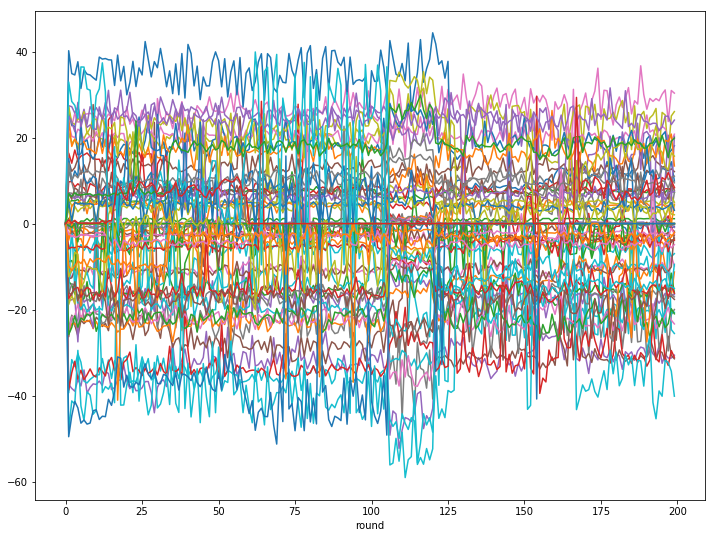
\includegraphics[width=0.75\textwidth]{h2startwealth.png}
  \caption{Wealth effect after each epoch for a typical, 64-agent example with the add-and-remove
    network update heuristic.}
  \label{h2startwealth}
\end{figure}

\begin{figure}
  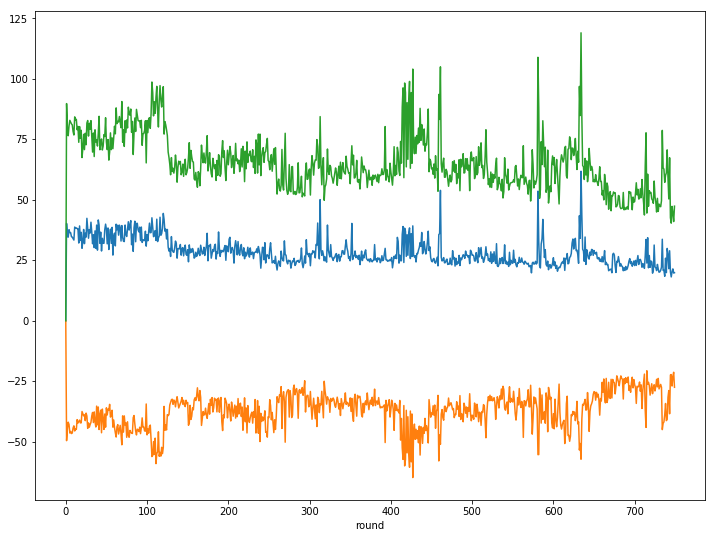
\includegraphics[width=0.75\textwidth]{h2startgap.png}
  \caption{Extrema of wealth effect after each epoch for a typical, 64-agent
    example with the add-and-remove network update heuristic. The maximum (blue),
    minimum (orange), and difference (green) for the first 800 epochs are shown.}
  \label{h2startgap}
\end{figure}

\begin{figure}
  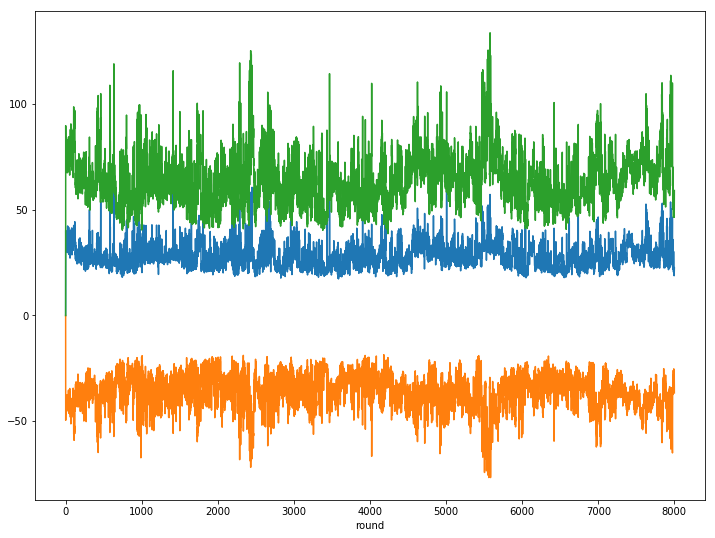
\includegraphics[width=0.75\textwidth]{h2allgap.png}
  \caption{Extrema of wealth effect after each epoch for a typical, 64-agent
    example with the add-and-remove network update heuristic. The maximum (blue),
    minimum (orange), and difference (green) for 8000 epochs are shown.}
  \label{h2allgap}
\end{figure}

\begin{figure}
  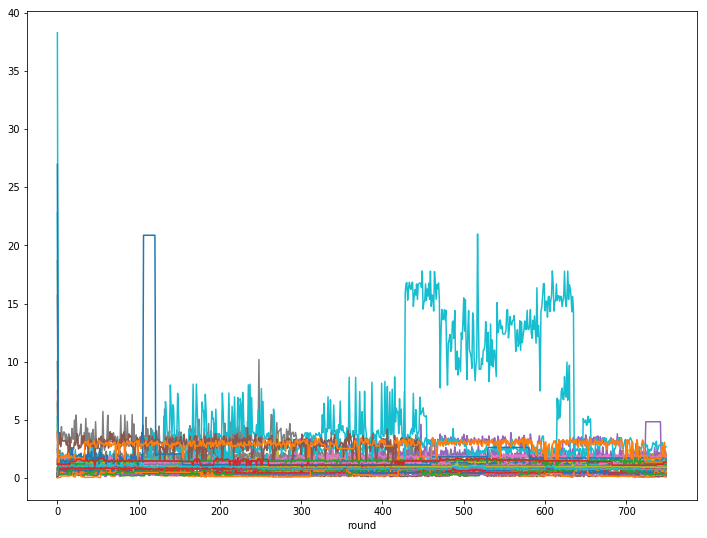
\includegraphics[width=0.75\textwidth]{h2prices.png}
  \caption{MRS of good two with respect to good one (numeraire) after each epoch
    for a typical, 64-agent example with the add-and-remove network update heuristic.
    Each color represents a different agent.}
  \label{h2prices}
\end{figure}

\begin{figure}
  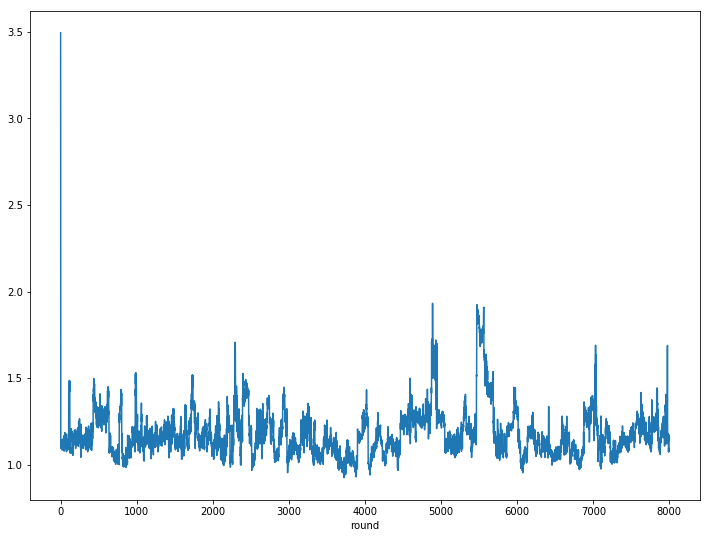
\includegraphics[width=0.75\textwidth]{h2allpriceave.png}
  \caption{Average MRS of good two with respect to good one (numeraire) after
    each epoch for a typical, 64-agent example with the add-and-remove network update heuristic. }
  \label{h2allpriceave}
\end{figure}

\section{Discussion}
Our results support the findings in \cite {wilhite2001bilateral}, i.e. that being positioned as a ``crossover'' node between otherwise
unconnected partitions of the trading network tends to improve the wealth change
outcome for that agent.
This same result has also been demonstrated more generally in that having more trading partners improved wealth change outcomes even if those new partners were well connected.
Additionally, it has been shown that modifying the trading network according to a
simple heuristic that considers wealth effect alone can achieve some measure of
convergence toward competitive equilibrium.
However, the simple heuristic adopted in this work did not converge
sufficiently to be used as an equilibrium-finding method. To that end, more work is needed to improve it.

First, it may be possible to use the wealth effect to make more efficient
choices for network modifications.
In the current model, new edges are created between the worst-off agent and
another agent chosen randomly with equal probability.
While this stochastic element was necessary to avoid cycling, it might be
improved by using the wealth effect data to construct a better distribution
from which to select the next agent.
Likewise for link removal, it may be possible to make better choices based on
wealth effect.

Second, the network update heuristic could be modified to account for the total
number of edges.
While it is desirable with respect to computational efficiency to avoid heuristics
that rely on the graph properties of network.
It is possible to keep a tally of the number of edges added or removed with
negligible computational resources.
With more research, it may be possible to combine this information with the
wealth effect results to improve the network update heuristic.

Third, a heuristic that explicitly prevents or otherwise accounts for
disconnected graph partitions should be developed. In the method described in
this work, it is unlikely but possible that a portion of the network could be
disconnected from the rest of the network. It is unclear if this is an issue
over many iterations, but for some rounds the result is that some small number
of agents do not make any trades. Obviously, no claim of finding competitive equilibrium
could be made under these circumstances. While traversing the graph to ensure
full connectivity would be inefficient. It may be possible to improve the
network update heuristic to prevent disconnected graphs.

Moreover, it will also be necessary to show that these, or any further results hold for an arbitrary number of goods.
Or, if analytical results are not forthcoming, that the method is
efficient for some useful number of goods.
Given that edges in the network are, by definition, bilateral, there is no reason to assume that economies with more than two goods share the same properties exploited by a network update
heuristic.

Finally, the results from \cite{sunder2002simple} might be incorporated in a
more direct way. It is likely that network updates alone may not suffice for
distributed agents to find competitive equilibrium with the desired precision or
efficiency at useful numbers of goods and agents. However, it may be possible to
combine the network modification strategies in this work with the price
information to realize the price subsidy approach of \cite{sunder2002simple}.
In this way, it may be possible to circumvent the cycling encountered when their
method is applied at scale.

\bibliographystyle{spbasic}
\bibliography{de}
\end{document}